%
% File naaclhlt2016.tex
%

\documentclass[11pt,letterpaper]{article}
\usepackage{naaclhlt2016}
\usepackage{times}
\usepackage{latexsym}
\usepackage{graphicx}
\usepackage{subcaption}

% \naaclfinalcopy % Uncomment this line for the final submission
\def\naaclpaperid{***} %  Enter the naacl Paper ID here

% To expand the titlebox for more authors, uncomment
% below and set accordingly.
% \addtolength\titlebox{.5in}    

\newcommand\BibTeX{B{\sc ib}\TeX}


\title{Crowd Knows Better: Crowdsourcing for Non-factoid Question Answering}

% Author information can be set in various styles:
% For several authors from the same institution:
% \author{Author 1 \and ... \and Author n \\
%         Address line \\ ... \\ Address line}
% if the names do not fit well on one line use
%         Author 1 \\ {\bf Author 2} \\ ... \\ {\bf Author n} \\
% For authors from different institutions:
% \author{Author 1 \\ Address line \\  ... \\ Address line
%         \And  ... \And
%         Author n \\ Address line \\ ... \\ Address line}
% To start a seperate ``row'' of authors use \AND, as in
% \author{Author 1 \\ Address line \\  ... \\ Address line
%         \AND
%         Author 2 \\ Address line \\ ... \\ Address line \And
%         Author 3 \\ Address line \\ ... \\ Address line}
% If the title and author information does not fit in the area allocated,
% place \setlength\titlebox{<new height>} right after
% at the top, where <new height> can be something larger than 2.25in

\author{Denis Savenkov \\ Emory University \\ {\tt dsavenk@emory.edu} 
  \And Scott Weitzner \\ Emory University \\ {\tt sweitzn@emory.edu}
  \And Eugene Agichtein \\ Emory University \\ {\tt eugene@mathcs.emory.edu}
}

\date{}

\begin{document}

\maketitle

\begin{abstract}
State the problem.
Why is it an interesting problem.
What is our contribution.
What are implications and value.
\end{abstract}

\section{Introduction}
\label{sec:introduction}

Describe the problem.
State contributions.

We focus on the following research questions:
\begin{enumerate}
\item RQ1. Can crowdsourcing be used to judge the quality of answers to non-factoid questions under time limit?
\item RQ2. Is it possible to use crowdsourcing to collect answers to real user questions under time limit?
\item RQ3. How the quality of crowdsourced answers to non-factoid question compare to original CQA answers and automatic answers from TREC LiveQA systems?
\end{enumerate}


\section{Methodology}
\label{sec:methodology}

\subsection{Crowdsourcing Interface}
\label{subsec:interface}



This section will describe the setup of our crowdsourcing experiments.




\section{Results}
\label{sec:results}

First, we will describe results on crowdsourcing answer ratings, because we are planning to use these scores to estimate the quality of generated answers.

\subsection{Answer validation}

To get ratings for answers and compare their quality against trained NIST assessors, we sampled 200 questions from TREC LiveQA 2015, and took answers from 3 different systems.
The interest of this work is in real-time scenario, therefore we made two experiments: with and without time pressure.
In the first experiment workers were given a minute to provide their judgments, and in the second experiment the working time wasn't limited.
Figure \ref{figure:score_correlation} shows correlation between official NIST assessor relevance judgments and ratings provided by our workers.
Results showed, that Pearson correlation between official scores and our ratings is $\rho=0.52$.
The distribution of scores shows, that official assessors were very generous in giving the lowest score of 1, mechanical turk scores tend to be a little higher and they assign extreme score less often.

However, in general, the results suggest that we can trust crowdsourced ratings and we will use them in our next experiment to estimate the quality of different answers.

\begin{figure}[t!]
	\centering
	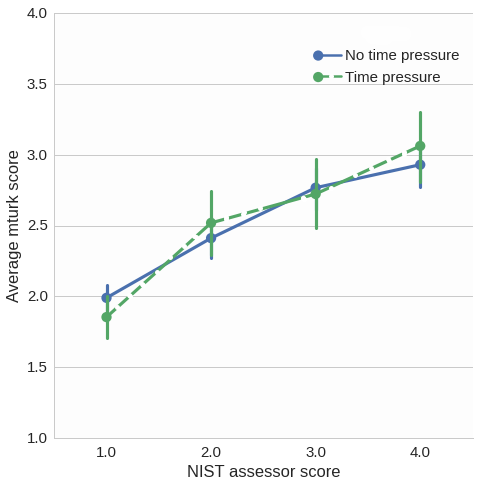
\includegraphics[width=0.5\textwidth]{img/score_correlation}
	\caption{Correlation between NIST assessor scores and crowdsourced ratings with and without time limit on the work time}
	\label{figure:score_correlation}
\end{figure}
	
Figure \ref{figure:validation_time} shows that even though the median time to rate all three answers is around 22-25 seconds in both experiments, the upper bound is significantly lower in the experiment with the time pressure.
	
\begin{figure}[t!]
	\centering
	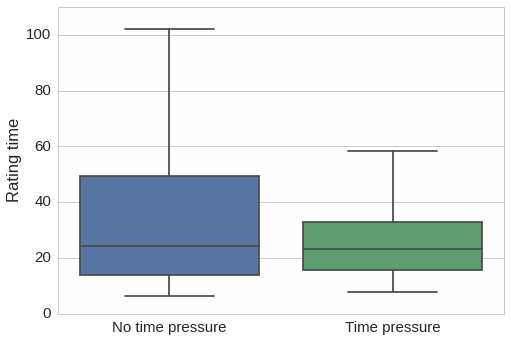
\includegraphics[width=0.5\textwidth]{img/validation_time}
	\caption{Box plot of rating time with and without time pressure}
	\label{figure:validation_time}
\end{figure}

\subsection{Answer crowdsourcing}

In the next experiment we asked Mechanical Turk workers to answer question from TREC LiveQA.
Again, we conducted two experiments with and without time restrictions.
In the first experiment users were given a minute to answer the given question and a countdown timer was displayed on the screen.
We collected 3 answers for each TREC LiveQA question.
Table \ref{table:answer_stats} summarizes some statistics on the answers.
First thing to notice is that, unlike CQA websites, where some questions are left unanswered, by paying the crowd workers we were able to get at least one answer for all LiveQA questions (after filtering ``NA'' and ``I don't know'' answers).
The length of the answers, provided by Mechanical turk users is lower, and time pressure forces user to be even more concise.


\begin{table}[h]
\centering
\caption{Statistics of different types of answers for Yahoo! Answers questions}
\begin{tabular}{| p{2.3cm} | c | c | c |}
\hline
Statistic & Y!A & mTurk & mTurk-time\\
\hline
\% answered & 78.7\% & 100.0\% & 100.0\% \\
Length (chars) & 354.96 & 190.83 & 126.65 \\
Length (words) & 64.54 & 34.16 & 22.82 \\
\hline
\end{tabular}
\label{table:answer_stats}
\end{table}

To answer RQ2 we took a sample of 100 LiveQA questions along with their original CQA, crowdsourced and some LiveQA participants answers and asked users to rate each of them on a scale from 1 to 4, similar to the official scoring.
Each set of answers was judged by 3 different workers, and their scores were averaged.
Figure \ref{fig:average_score} displays the plot with average score for answers from different sources.
Quite surprisingly the quality of collected answers turned out be comparable to answers provided by the CQA website users.
Average rating of answers produced by the winning TREC LiveQA system is also pretty close to those of human answers.
Finally, as expected, time pressure had its negative effect on the quality.

\begin{figure}[h]
	\centering
	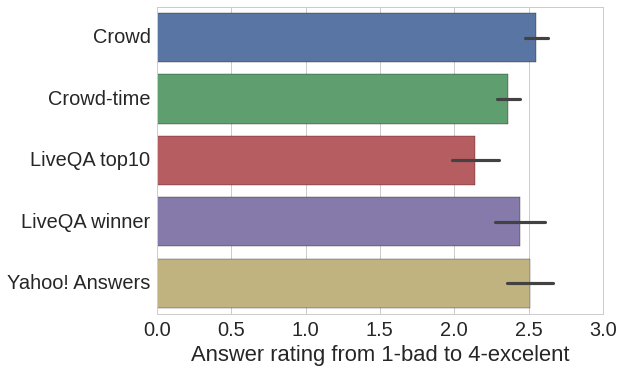
\includegraphics[width=0.5\textwidth]{img/average_score}
	\caption{Average scores of different type of answers to Yahoo! Answers questions for different categories}
	\label{fig:average_score}
\end{figure}

Analysis of scores distribution (Figure \ref{fig:scores_distribution}) shed some light on the nature of the problems with automatic and human answers.
As we can see, automatic systems generate non-relevant answers ($score=1$) more often than human.
This means, that quite often the model either fails to retrieve relevant information or to separate between useful and non-useful answer candidates.
However, by having larger information store, e.g. world wide web, question answering systems can often find the perfect answer ($score=4$), while regular people tend to give generally useful responses ($score=2,3$).

\begin{figure}[h]
\centering
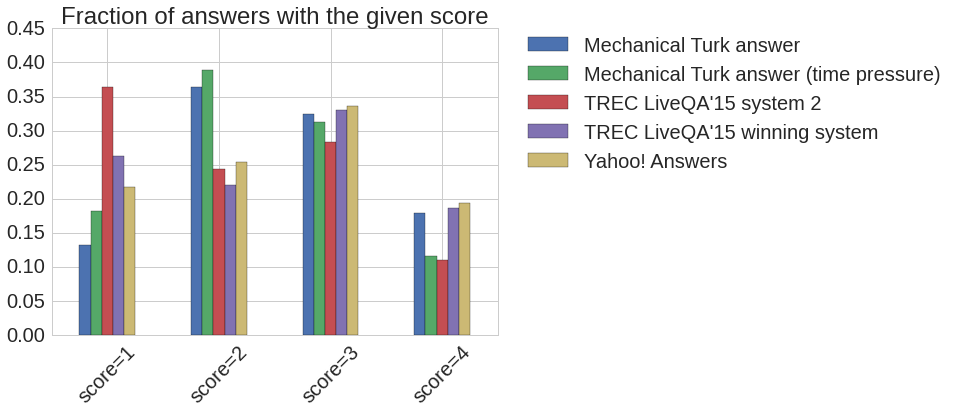
\includegraphics[width=0.5\textwidth]{img/scores_distribution}
\caption{Distribution of scores for different types of answers to Yahoo! Answers questions}
\label{fig:scores_distribution}
\end{figure}

From Figure \ref{fig:answering_time_distribution} we can see that adding time pressure shifts the distribution of answering times\footnote{For the experiment with time pressure we had separate timers for reading instructions, reading the question and writing the answer, that's why the total time on the plot could be more than 1 minute}.

\begin{figure}[h]
	\centering
	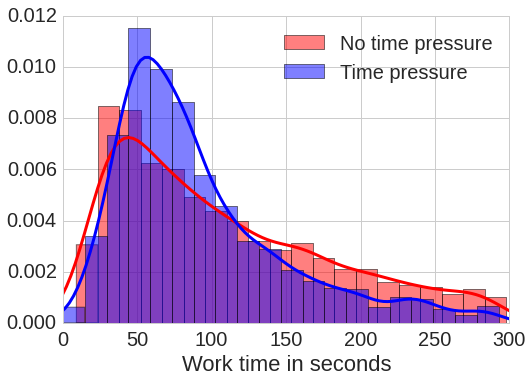
\includegraphics[width=0.5\textwidth]{img/answering_time_distribution}
	\caption{Distribution of answering times for experiments with and without time pressure}
	\label{fig:answering_time_distribution}
\end{figure}


\section{Discussion}
\label{sec:discussion}

Some discussion on the results and possible future work.

\section{Related Work}
\label{sec:related_work}

In \cite{bernstein2012direct} authors used a combination of log mining and crowdsourcing to build answers to a long tail of questions, that search engine users ask, therefore increasing the coverage of direct answers

\section{Conclusion}
\label{sec:conclusion}

Final words.

\section*{Acknowledgments}

If any...

\bibliography{naaclhlt2016}
\bibliographystyle{naaclhlt2016}


\end{document}
